\documentclass[12pt,letterpaper]{article}
\usepackage[utf8]{inputenc}
\usepackage[english]{babel}
\usepackage{amsmath}
\usepackage{amsfonts}
\usepackage{amssymb}
\usepackage{graphicx}
\usepackage{caption}
\usepackage{subcaption}
\usepackage[left=2cm,right=2cm,top=2cm,bottom=2cm]{geometry}
\author{White Team \\ Chenxi Rong, Xiaoquan Liu, Zhanyi Lin, Fabian Schmid}
\title{Estimate the Impact of Opioid Control Policies \\ (Report for Nick)}
\begin{document}
\maketitle

\section{Motivation}
Opioids are a class of drugs that include prescription opioids (natural and semi-synthetic opioids and methadone), heroin, and synthetic opioids other than methadone (primarily fentanyl) that derive from, or mimic, natural substances found in the opium poppy plant and work in the brain to produce a variety of effects, including pain relief. Opioid drugs include prescription pain medicine and illegal drugs. Some people may experience euphoria, a joyful sensation of well-being, from opioids, whether they are legally prescribed or not. Opioids do not always generate euphoria, but for those who do, there is a chance they will be used again and again because of how they feel. Therefore, even with a doctor's supervision, using opioids can pose risks. A person's tolerance and dependency to prescription drugs can develop over time, necessitating greater and more frequent dosages, finally leading to addiction and the person's turning to illegal markets in order to maintain their addiction, and subsequently causing death.

According to the Centers for Disease Control and Prevention (CDC), the number of drug overdose deaths has quintupled since 1999, and the rise in opioid overdose deaths can be outlined in three distinct waves: the first wave in the 1990s with increased prescribing of opioids, the second wave in 2010 with heroin, and the third wave in 2013 with synthetic opioids like fentanyl. In order to fight the opioid overdose epidemic, policymakers have made policy interventions to limit the over prescription of opioids. Texas regulations with regard to treating pain with controlled substances went into effect in January 2007. Florida’s legislature became effective in 2010, and a series of changes related to drug prescription took place in the following years. Washington regulated the prescribing requirements of opioids for pain treatment in January 2012, which included periodic patient reviews, milligram thresholds, strict documentation guidelines, and consultations with pain management experts.

For all three of these policy changes, we performed both a pre-post analysis and a difference-in-difference analysis to understand the effect of opioid drug regulations on both the amount of opioid shipments and drug overdose deaths. For the pre-post analysis, we will demonstrate the trend of overdose deaths and opioid shipments over years. After the policy went into effect, we analyze if our plots show a difference in the trend in each state compared to the years before the policy implementation.

However, to further valid our analysis of causation between opioid drug regulations and both the amount of opioids shipments and drug overdose deaths, we need to eliminate the effect of confounders. For example, the US Customs Service managed to dramatically reduce the importation of fentanyl into the United States at the same time Florida’s policy went into effect, which would likely reduce the number of overdose deaths throughout the United States. If we were just to use the pre-post analysis to bring a conclusion by comparing Florida in 2009 to Florida in 2011, we would wrongly attribute the decline in the amount of shipments and overdose deaths to Florida’s policy change. With a difference-in-difference analysis, we use the observed outcomes of people who are exposed to drug regulations (i.e., data from Texas, Florida, and Washington) and people who were not exposed to drug regulations (i.e., for each of those states, we picked three states as comparison states) both before and after the policy went into effect. We compare the development in the treatment and control states over time to evaluate the impact of opioid control policies. A crucial assumption is that the trend in the control states after the policy implementation is similar to the one that the treatment state would have experienced without the policy. For that, it is necessary that the control states have similar characteristics as the treated state so that a potential change in trends can only be explained by the policy.

\section{Data}
We used drug overdose death data from the US Vital Statistics records, prescription opioid drug shipments from the Washington Post, FIPS codes based on a file from the US Census, and US census population data. All these data sets need at least a location name (to infer the county) and a temporal unit (to infer the year). All raw data was aggregated at the county-year level so that the data is available for our preferred unit of observation.

For the opioid shipment data, we used the total active weight of the drug in grams and converted it to a morphine equivalent so that different kind of opioids are comparable. To deal with the huge raw data set ($>$ 100 GB), we only imported the required columns, chunked the data, and grouped it by year and county to reduce the number of rows and end up with our preferred unit of observation in a smaller data set. After the chunking process, it was necessary to group again by year and county so that there is only one observation per year and county in the final data set. This assumption was successfully tested with the assert statement. Unfortunately, this data set only contains the county name but no FIPS code. This problem was solved later in the merging step.

For the mortality data, we assigned the following five death causes as drug related: "Drug poisonings (overdose) Undetermined (Y10-Y14)", "Drug poisonings (overdose) Unintentional (X40-X44)", "Drug poisonings (overdose) Suicide (X60-X64)", "Drug poisonings (overdose) Homicide (X85)", and "All other drug-induced causes". Again the FIPS code caused problems in this data set. Although they were already included, some of them had only four digits so that it was required to add a zero in front of these cases so that the merging later on works without problems.

The US census population data is published once every decade. As we require data for two decades, we used two datasets and concatenated them. The population data set also required modifications to the FIPS code as it only included the two-digit state FIPS code and the three-digit county FIPS code. To combine them, it was again necessary to add zeros in the front if the code has only one or two digits. Furthermore, it was necessary to reshape the data from wide to long so that we have our preferred unit of observation.

Based on our research questions and data collected, we merged the imported and cleaned raw data into two master sheets. The first one contains opioid shipment and population to analyze how the policy influences the amount of shipped opioid. The second one contains the overdose death data and population data. 

The different data sets were merged based on the county FIPS codes and the year. FIPS codes are already included in the population data set and the US Vital Statistics records. Because the opioid shipment data only contains the county name and state name, but no FIPS code, we merge this dataframe with a data set including all county FIPS codes and the associated county and state name. At first, the merging process generated some observations with no FIPS code. With the option indicators, we found that this is caused by the different spellings of the county name in the FIPS data and in the opioid shipment data. After unifying the spelling of the county names in both dataframes, the merge succeeded with a m:1 pattern. This was successfully tested with an assert statement.

In the next step, we merge the intermediate dataframe with the population data based on the FIPS code and year since the data is grouped by our preferred unit of observation. After the merge, we found that there are opioid shipment data only observations. We checked the specific counties and states which miss the population data. The output indicated that the counties which have no population data are in Puerto Rico which is a Caribbean Island and an unincorporated U.S. territory island. This state is not one of our target analysis states or in our selected control group. Hence, we safely drop these counties.

As both the master sheet for overdose death and population have the variables FIPS and year, we directly merge them based on these two features. We also employed the option indicator and validate to check the merge results. Firstly, the validate option showed that the observations are merged in m:1 pattern. However, the indicator returns that in addition to AK, there are still two counties in VA with missing population data. We examined the population data of those two counties and found the population data does not include those two counties. As we discussed in the former part, Virginia is also not needed in our analysis. Hence, we currently drop these observations. If these counties are needed for future analysis, we will use other sources to find the corresponding population of these two counties.

\section{Analysis}

\subsection{Summary statistics}
As described, the analysis takes a look at two outcome variables. In Table \ref{tab:sum_deaths}, summary statistics for overdose deaths per 100,000 people are provided. They are reported separately for states with policy changes and the corresponding control group before and after the policy implementation.

\begin{table}[!h]\centering \caption{Summary statistics for overdose deaths per 100,000 inhabitants \label{tab:sum_deaths}}

\begin{tabular}{ccccccc}\hline \hline
 State & \begin{tabular}[x]{@{}c@{}}Year of policy\\implementation\end{tabular}& Statistics & Mean & Std. Dev. & Min. & Max. \\ \hline
Florida & 2010 & Before & 14.57 & 6.13 & 3.83 & 35.19 \\
 & & After & 14.92 & 6.35 & 3.90 & 40.82 \\
Control group (NC, TN, IA) & & Before & 14.15 & 7.48 & 3.33 & 46.91 \\
 & & After & 17.73 & 9.51 & 4.95 & 67.67 \\ \hline
Texas & 2007 & Before & 10.14 & 6.57 & 1.46 & 41.55 \\
 & & After & 10.38 & 4.99 & 1.80 & 35.45 \\
Control group (WV, OR, ID) & & Before & 17.29 & 13.25 & 3.56 & 61.83 \\
 & & After & 30.22 & 24.63 & 3.39 & 123.61 \\ \hline
Washington & 2012 & Before & 13.28 & 5.36 & 4.26 & 31.41 \\
 & & After & 13.97 & 4.75 & 5.68 & 26.39 \\ 
Control group (KS, NJ, OR) & & Before & 9.47 & 5.04 & 1.56 & 28.02 \\
 & & After & 13.21 & 5.91 & 3.39 & 30.37 \\

\end{tabular}

\end{table}


Table \ref{tab:sum_ship} summarizes the statistics for the opioid shipment data. Data for Texas is not reported as a different approach was required for this state. Due to the unavailability of enough annual data prior to the policy change, the analysis in Texas is conducted on a monthly basis.

\begin{table}[htbp]\centering \caption{Summary statistics for opioid shipments in MME converted grams per capita \label{tab:sum_ship}}

\begin{tabular}{ccccccc} \hline \hline
State & \begin{tabular}[x]{@{}c@{}}Year of policy\\implementation\end{tabular} & Statistics & Mean & Std. Dev. & Min. & Max. \\ \hline
Florida & 2010 & Before & 0.45 & 0.28 & 0.08 & 1.78 \\
& & After & 0.53 & 0.33 & 0.07 & 2.27 \\
Control group (TN, WV, NV) & & Before & 0.51 & 0.34 & 0.00 & 2.56 \\
& & After & 0.71 & 0.42 & 0.03 & 2.51 \\
Washington & 2012 & Before & 0.36 & 0.16 & 0.10 & 0.85 \\
& & After & 0.39 & 0.15 & 0.14 & 0.88 \\
Control group (IL, WI, RI) & & Before & 0.20 & 0.11 & 0.00 & 0.92 \\
& & After & 0.25 & 0.13 & 0.00 & 1.08
\end{tabular}
\end{table}

\subsection{Florida}

\textbf{Opioid shipments}

\begin{figure}[!h]
\centering
\begin{subfigure}{.5\textwidth}
  \centering
  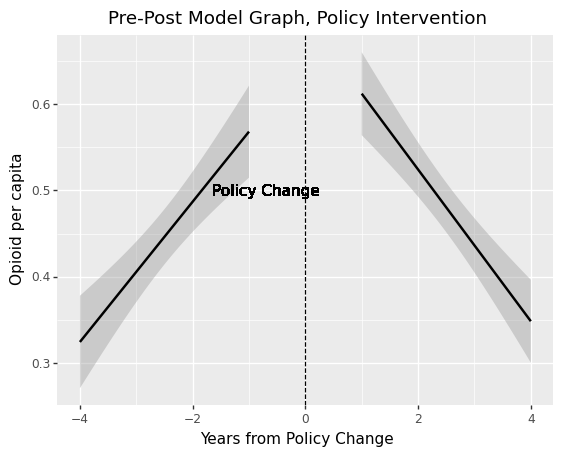
\includegraphics[width=.9\linewidth]{../30_results/General_Results/florida_opioid_shipment_prepost.png}
  \caption{Pre-post analysis}
  \label{fig:fl_ship_prepost}
\end{subfigure}%
\begin{subfigure}{.5\textwidth}
  \centering
  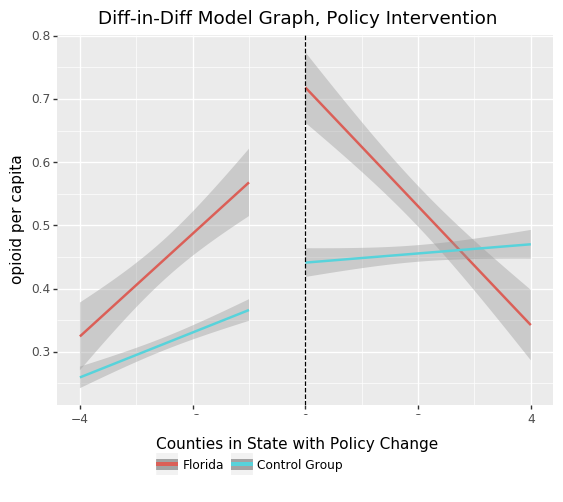
\includegraphics[width=.9\linewidth]{../30_results/General_Results/florida_opioid_shipment_diffdiff.png}
  \caption{Diff-in-diff analysis}
  \label{fig:fl_ship_did}
\end{subfigure}
\caption{Analysis of opioid policy on opioid shipments in Florida}
\label{fig:fl_ship}
\end{figure}

From the output of the pre-post graph in Figure \ref{fig:fl_ship}, we can see the slope of the regression model of opioid shipments per capita. The slope was positive before the policy became effective, but changed to negative after the date the policy became effective. This means that the opioid shipments per capita increased year by year before the policy change and started to decrease annually after the policy was rolled out. Therefore, we may conclude that the policy is effective in Florida in reducing opioid shipments according to the pre-post analysis.

For the different-in-different analysis, we selected Georgia, North Carolina, and South Carolina for the control groups since those three states are close to Florida. From the output, we can see that after the policy implementation the slope of the control group is still positive but the slope of Florida's opioid shipment converts to negative. For that reason, we infer that the decrease of the opioid shipments per capita in Florida after 2010 is caused by the policy, which implies that the policy is effective. \\

\noindent \textbf{Overdose deaths} \\

\begin{figure}[!h]
\centering
\begin{subfigure}{.5\textwidth}
  \centering
  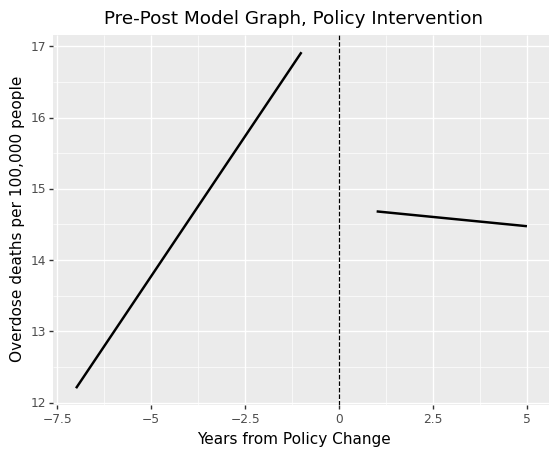
\includegraphics[width=0.7\linewidth]{../30_results/General_Results/florida_overdose_death_prepost.png}
  \caption{Pre-post analysis}
  \label{fig:fl_death_prepost}
\end{subfigure}%
\begin{subfigure}{.55\textwidth}
  \centering
  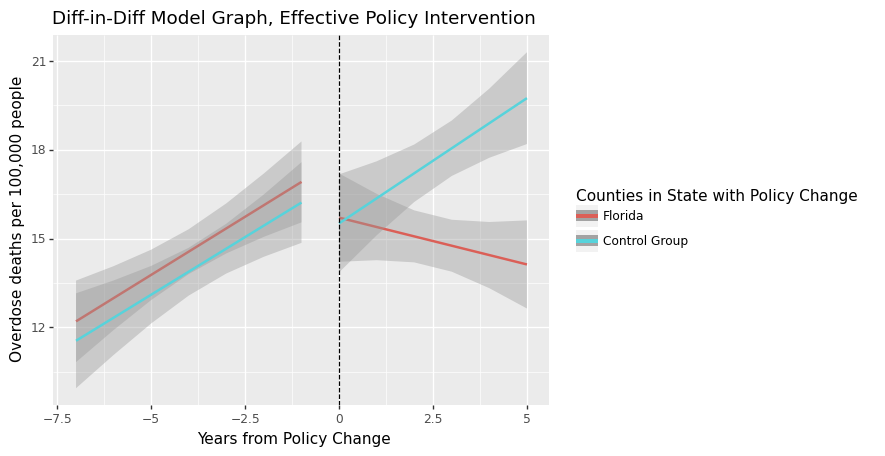
\includegraphics[width=1\linewidth]{../30_results/General_Results/florida_overdose_death_diffdiff.png}
  \caption{Diff-in-diff analysis}
  \label{fig:fl_death_did}
\end{subfigure}
\caption{Analysis of opioid policy on overdose deaths in Florida}
\label{fig:fl_death}
\end{figure}


Now, the impact on overdose deaths per 100,000 inhabitants is analyzed. The pre-post graph in Figure \ref{fig:fl_death} shows that there was a positive trend before the policy became effective, but it switched to negative after the date the policy became effective. This means that the overdose deaths per capita increased year by year before the policy change and started to decrease annually after the policy effective date. Therefore, we may conclude that the policy is effective in Florida according to the pre-post analysis. The difference-in-difference analysis shows that before the policy, Florida and the control groups had a similar increasing trend in overdose deaths. However, we witness that after the policy went into effect the overdose deaths in states of the control group are still increasing but the slope of Florida overdose deaths per 100,000 inhabitants is actually decreasing. Hence, the diff-in-diff results confirm our initial conclusion of the pre-post analysis that the policy is effective in reducing overdose deaths in Florida.

\subsection{Texas}
\textbf{Opioid shipments}

\begin{figure}[!h]
\centering
\begin{subfigure}{.5\textwidth}
  \centering
  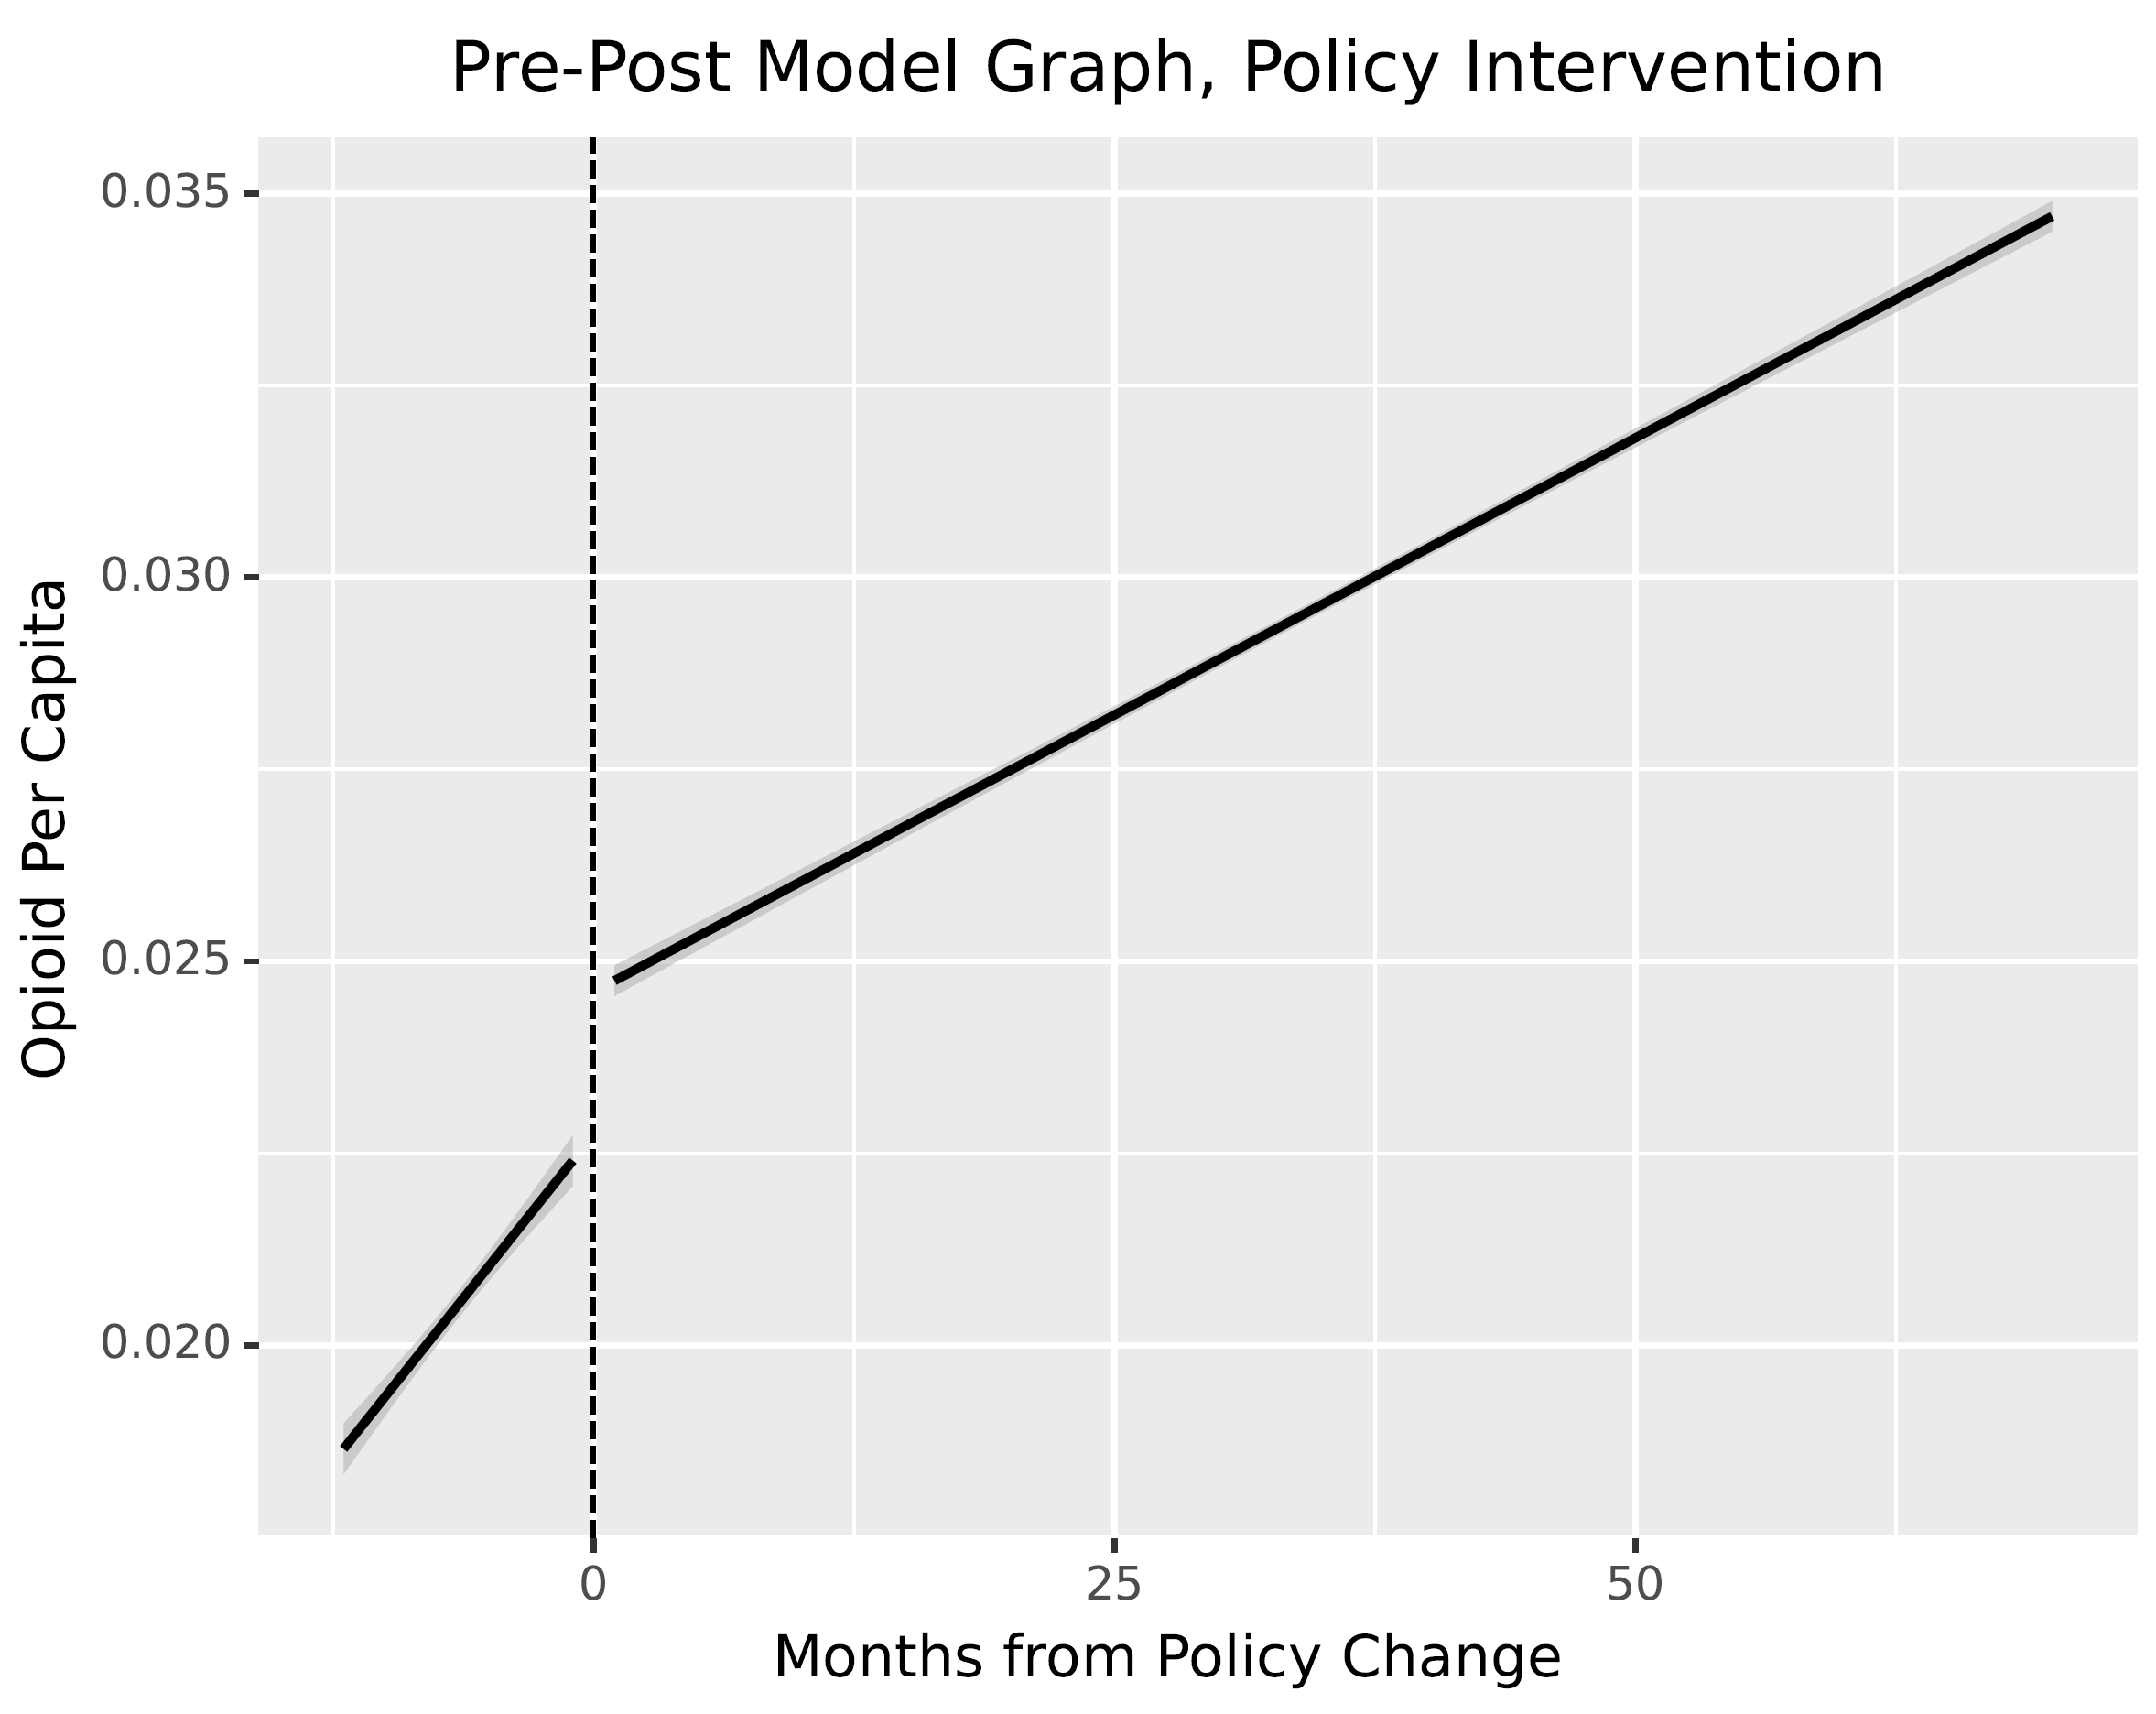
\includegraphics[width=0.7\linewidth]{../30_results/Bonus_Results/tx_monthly_prepost_successful.png}
  \caption{Pre-post analysis}
  \label{fig:tx_ship_prepost}
\end{subfigure}%
\begin{subfigure}{.55\textwidth}
  \centering
  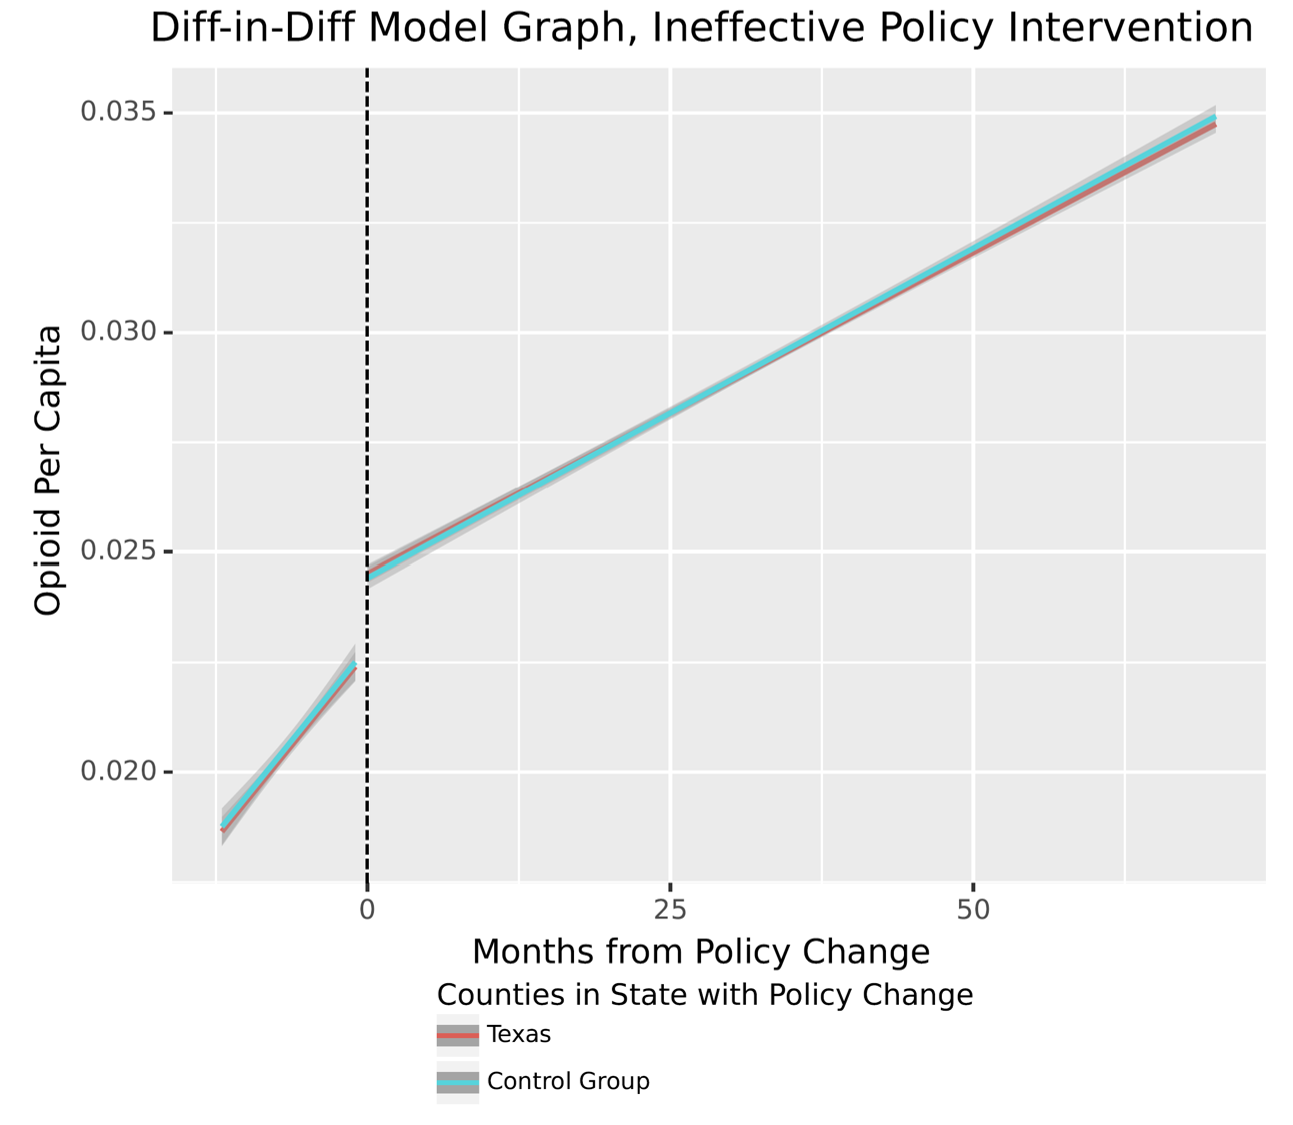
\includegraphics[width=0.7\linewidth]{../30_results/Bonus_Results/tx_monthly_did_notsure.png}
  \caption{Diff-in-diff analysis}
  \label{fig:tx_ship_did}
\end{subfigure}
\caption{Analysis of opioid policy on opioid shipments in Texas}
\label{fig:tx_ship}
\end{figure}
Since our shipment data only runs from 2006, meaning we only have one year of data before the policy change, we analyzed opioid shipment data by month instead of by year. In the left part of the pre-post chart in Figure \ref{fig:tx_ship}, the slope is sharper than on the right, which implies that the prescription opioid shipment amount per capita increased month by month in Texas before January 2007. After the policy became effective in January 2007, the trend is still increasing, but the gradient is smaller. Therefore, we may conclude that the policy restricted the opioid shipments by a small amount.

For the difference-in-difference analysis, we selected Arkansas, Oklahoma, and New Mexico as states for the control group since these three states are close to Texas. The two almost parallel lines before the policy intervention confirm the common trend assumption. After the policy implementation, the trend in Texas and the control states is still similar. Thus, we cannot confirm that the opioid policy was successful in controlling the opioid shipments in Texas. \\

\noindent \textbf{Overdose deaths}

\begin{figure}[!h]
\centering
\begin{subfigure}{.5\textwidth}
  \centering
  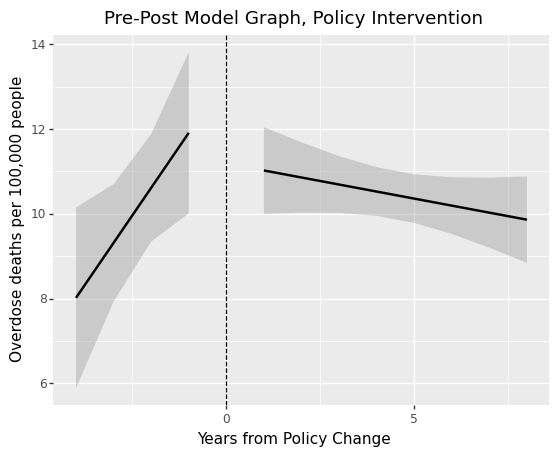
\includegraphics[width=0.7\linewidth]{../30_results/General_Results/texas_overdose_death_prepost.png}
  \caption{Pre-post analysis}
  \label{fig:tx_death_prepost}
\end{subfigure}%
\begin{subfigure}{.55\textwidth}
  \centering
  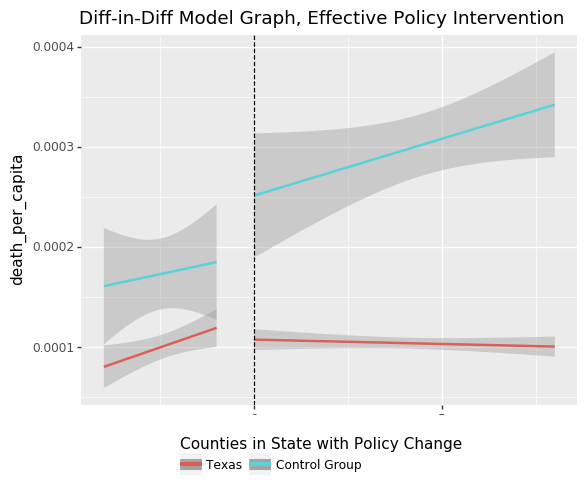
\includegraphics[width=1\linewidth]{../30_results/General_Results/texas_overdose_death_diffdiff.png}
  \caption{Diff-in-diff analysis}
  \label{fig:tx_death_did}
\end{subfigure}
\caption{Analysis of opioid policy on overdose deaths in Texas}
\label{fig:tx_death}
\end{figure}

From the pre-post graph in Figure \ref{fig:tx_death}, we can infer that the slope for overdose deaths per 100,000 people was positive before the policy became effective, but changed to negative after that in 2007. This implies that the overdose death per 100,000 inhabitants increased year by year before the policy change and started to decrease annually after the policy's effective date. Therefore, we can conclude that the policy is effective in Texas according to the pre-post analysis. The difference-in-difference analysis shows that the slope of  the control group is still positive, but the slope for Texas converts to negative. For that, we gathered evidence that the policy was successful in reducing overdose deaths in Texas.

\subsection{Washington}
\textbf{Opioid shipments}

\begin{figure}[!h]
\centering
\begin{subfigure}{.5\textwidth}
  \centering
  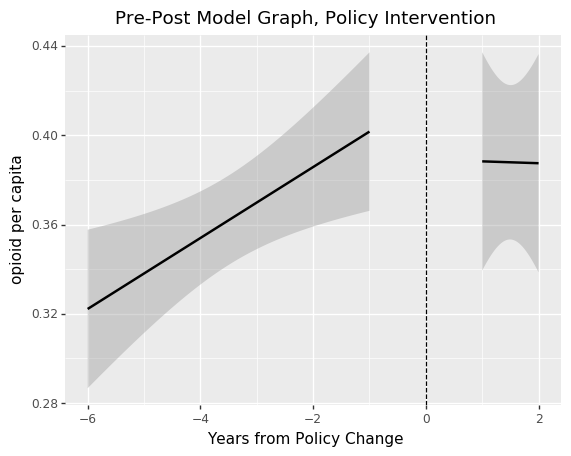
\includegraphics[width=0.7\linewidth]{../30_results/General_Results/washington_opioid_shipment_prepost.png}
  \caption{Pre-post analysis}
  \label{fig:wa_ship_prepost}
\end{subfigure}%
\begin{subfigure}{.55\textwidth}
  \centering
  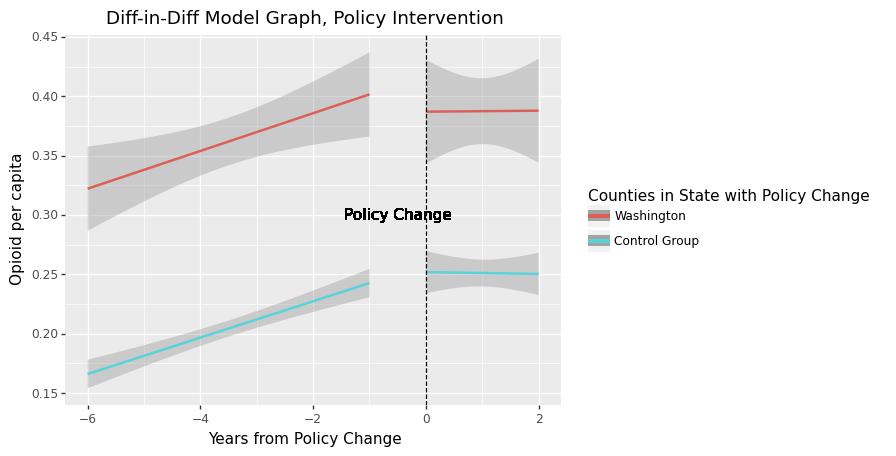
\includegraphics[width=1\linewidth]{../30_results/General_Results/washington_opioid_shipment_diffdiff.png}
  \caption{Diff-in-diff analysis}
  \label{fig:wa_ship_did}
\end{subfigure}
\caption{Analysis of opioid policy on opioid shipments in Washington}
\label{fig:wa_ship}
\end{figure}

The pre-post plot highlights that the slope of prescription opioid shipments was positive before the policy became effective in Washington in 2012. It is slightly negative after the policy implementation. Even though the gradient indicates that the decreasing speed is not high, the overall trend is totally different from the previous years. Hence, we infer that the policy has a negative influence on the number of shipped prescription opioids.

For the difference-in-difference analysis, we selected Oregon, Idaho, and Montana as control groups since those three states are close to Texas. From the output, we can see the gradient change is similar for Washington and for the states in the control group. Hence, we have no evidence that the policy is the only factor which deceased the prescription opioid shipment amount per capita. \\

\noindent \textbf{Overdose deaths}

\begin{figure}[!h]
\centering
\begin{subfigure}{.5\textwidth}
  \centering
  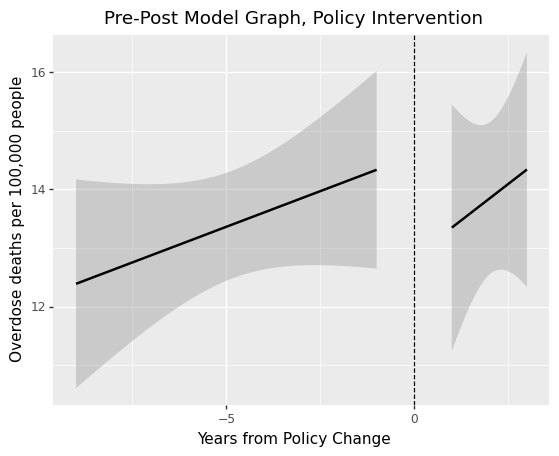
\includegraphics[width=0.7\linewidth]{../30_results/General_Results/washington_overdose_death_prepost.png}
  \caption{Pre-post analysis}
  \label{fig:wa_death_prepost}
\end{subfigure}%
\begin{subfigure}{.55\textwidth}
  \centering
  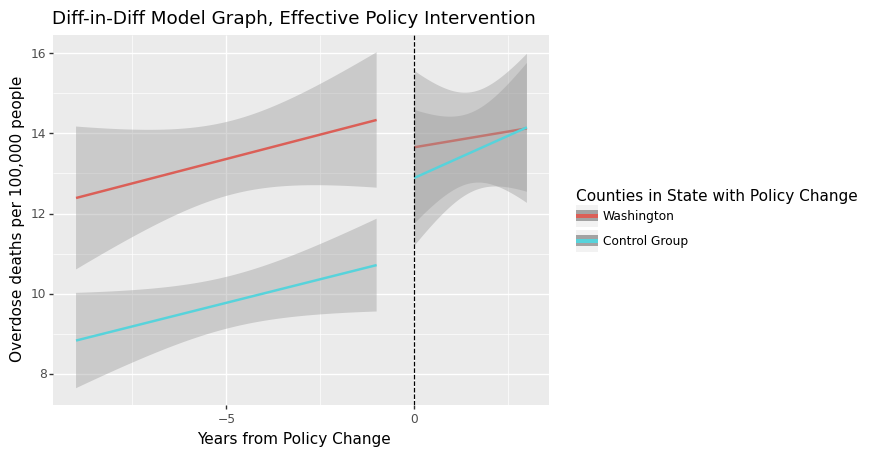
\includegraphics[width=1\linewidth]{../30_results/General_Results/washington_overdose_death_diffdiff.png}
  \caption{Diff-in-diff analysis}
  \label{fig:wa_death_did}
\end{subfigure}
\caption{Analysis of opioid policy on overdose deaths in Washington}
\label{fig:wa_death}
\end{figure}

From the output of the pre-post graph, we can tell that the slope for overdose deaths per 100,000 people was both positive before and after the policy became effective. Though briefly after the policy became effective, the overdose death per capita became lower, the overdose death per capita still increased year by year after the policy's effective date. Besides that, the difference-in-difference analysis indicates that the trends for both Washington and states in the control group are the same before and after the policy became effective. Therefore, our evaluation implies that the policy did not achieve a change in overdose death numbers in Washington.


\section{Conclusion}

Assuming that the above mentioned assumptions for the pre-post and difference-in-difference analysis are met, we can summarize the causal impact of the opioid policies on opioid shipments and overdose deaths in three US states. Based on the graphs of our pre-post and difference-in-difference analysis, Florida's drug policy was effective in decreasing the prescription opioid shipment amount as well as decreasing the overdose deaths. Texas' drug policy was not successful in controlling the opioid shipments but did decrease the overdose deaths. However, Washington's drug policy was not successful in both controlling the opioid shipments and decreasing the overdose deaths.




\end{document}
